\documentclass[%
]{beamer}
\usepackage{graphicx} % For including single page pdfs
\usepackage{bm}       % bold math
\usepackage{pgffor}   % for loop
\usepackage{tikz}
\usepackage{multimedia}
\usepackage{layouts}
\usepackage{hyperref}
\usepackage{cambridge_lecture}

\usepackage{calculator}

\newcommand{\cols}[3][0.5]{%
    \SUBTRACT{1.}{#1}{\wdthb}
    \begin{columns}
        \begin{column}{#1\textwidth}
            #2
        \end{column}
        \begin{column}{\wdthb\textwidth}
            #3
        \end{column}
    \end{columns}
}

\newcommand{\figname}{}
\newenvironment{figright}[2][0.5]{%
    \renewcommand{\figname}{#2}
    \SUBTRACT{1.}{#1}{\wdthb}
    \begin{columns}
        \begin{column}{#1\textwidth}
        }{%
        \end{column}
        \begin{column}{\wdthb\textwidth}
            \includegraphics[width=\textwidth]{\figname}
        \end{column}
    \end{columns}
}

\newcommand{\dfigname}{}
\newenvironment{dfigright}[3][0.5]{%
    \renewcommand{\figname}{#2}
    \renewcommand{\dfigname}{#3}
    \SUBTRACT{1.}{#1}{\wdthb}
    \begin{columns}
        \begin{column}{#1\textwidth}
        }{%
        \end{column}
        \begin{column}{\wdthb\textwidth}
            \includegraphics[width=\textwidth]{\figname}
            \includegraphics[width=\textwidth]{\dfigname}
        \end{column}
    \end{columns}
}



\newenvironment{figleft}[2][0.5]{%
    \SUBTRACT{1.}{#1}{\wdthb}
    \begin{columns}
        \begin{column}{#1\textwidth}
            \includegraphics[width=\textwidth]{#2}
        \end{column}
        \begin{column}{\wdthb\textwidth}
        }{%
        \end{column}
    \end{columns}
}

\newenvironment{dfigleft}[3][0.5]{%
    \SUBTRACT{1.}{#1}{\wdthb}
    \begin{columns}
        \begin{column}{#1\textwidth}
            \includegraphics[width=\textwidth]{#2}
            \includegraphics[width=\textwidth]{#3}
        \end{column}
        \begin{column}{\wdthb\textwidth}
        }{%
        \end{column}
    \end{columns}
}


\newcounter{numimages}

\newenvironment{multifig}[1]{%
    \begin{frame}
        \pdfximage{#1}%
        \setcounter{numimages}{\the\pdflastximagepages}
        \addtocounter{numimages}{-1}

        \begin{tikzpicture}[remember picture, overlay]
            \foreach \pagenum in {1,...,\thenumimages} {%
                \node<handout:0|beamer:\pagenum>[anchor=center] at (current page.center) {
                \includegraphics[width=\textwidth,page=\pagenum]{#1}}; 
            }
            \addtocounter{numimages}{1}
            \node<handout:1|beamer:\thenumimages>[anchor=center] at (current page.center) {
            \includegraphics[width=\textwidth,page=\thenumimages]{#1}}; 
        \end{tikzpicture}
    }{%
    \end{frame}
}

\usepackage{layouts}



\title{Curvature tension}
\subtitle{Evidence for a closed universe (?)}
\author[Handley] % (optional, for multiple authors)
{Will Handley\\ \small{wh260@cam.ac.uk}}
\institute[University of Cambridge] % (optional)
{%
    Astrophysics Group, Cavendish Laboratory, University of Cambridge\\
    Kavli Institute for Cosmology, Cambridge\\
    Gonville \& Caius college, Cambridge\\
}
\date{25\textsuperscript{th} August 2019}

% Abstract
% --------
% Observational cosmology is close to breaking point. There is now a 4.9-sigma
% tension between the expansion rate $H_0$ as inferred by CMB modelling and
% $H_0$ as measured by supernovae observers. Other parameter tensions
% potentially exist between alternative combinations of data, such as a DES and
% Planck ($S_8$ and $\Omega_m$), or Planck CMB and lensing ($\Omega_K$). In
% these cases it is less obvious how to quantify the level of tension in terms
% of ``sigma'', either due to the high dimensionality of the space, or the
% non-gaussianity of the distributions. Diagnosing the location and level of
% these tensions could prove critical in determining their cause.
%
% In this talk I will discuss recent research by Pablo Lemos and myself into
% novel statistical ways to measure these tensions, how to quantify the number
% of parameters a given experiment constrains, the calibration of the DES
% evidence ratio and the problems with principle component analysis (PCA).


\begin{document}

\begin{frame}
    \titlepage{}
    \begin{center}
        Handley \arxiv{1908.09139}, \arxiv{1907.08524}\\
        Handley \& Lemos \arxiv{1902.04029}, \arxiv{1903.06682}

    \vspace{10pt}
    \url{github.com/williamjameshandley/CosmoChord}
    \url{github.com/williamjameshandley/anesthetic}
    \end{center}
\end{frame}

\begin{frame}
    \frametitle{Outline}
    \framesubtitle{A talk of two halves}
    \begin{description}
        \item[First half:] Inference, quantifying tensions and observing curvature
        \item[Second half:] Theory and predictions of primordially curved universes
    \end{description}
\end{frame}

\begin{frame}
    \frametitle{The Hubble $H_0$ tension}
    \begin{columns}
        \begin{column}{0.5\textwidth}
        \begin{itemize}
            \item CMB cosmologists (Planck) infer \\ $H_0=67\pm0.5\text{ km s}^{-1} \text{Mpc}^{-1}$
            \item Supernovae data  ($SH_0ES$) measure \\ $H_0=74\pm1.4 $
            \item $>4\sigma$ discrepancy could be due to:
                \begin{itemize}
                    \item Systematic error
                    \item Problem with standard model of cosmology ($\Lambda$CDM)
                \end{itemize}
            \item Inconsistent datasets shouldn't be combined
        \end{itemize}
        \end{column}
        \begin{column}{0.5\textwidth}
            \begin{overlayarea}{\textwidth}{0.5\textheight}
            \includegraphics<1>{./plots/H0.pdf}
            \includegraphics<2>{./plots/H0_combined.pdf}
            \end{overlayarea}
        \end{column}
    \end{columns}
\end{frame}


\begin{frame}
    \frametitle{$\sigma_8$-$\Omega_m$ tension}
    \begin{columns}
        \begin{column}{0.5\textwidth}
        \begin{itemize}
            \item<1-> Matter density $\Omega_m$ and RMS matter fluctuations $\sigma_8$ are constrained by 
            \item<1-> BAO and Planck look consistent
            \item<2-> DES is less clear
            \item<2-> How do you define a tension in terms of ``sigma'' for this case?
        \end{itemize}
        \end{column}
        \begin{column}{0.5\textwidth}
            \begin{overlayarea}{\textwidth}{0.5\textheight}
            \includegraphics<1>{./plots/BAO_planck.pdf}
            \includegraphics<2>{./plots/DES_planck.pdf}
            \end{overlayarea}
        \end{column}
    \end{columns}
\end{frame}

\begin{frame}
    \frametitle{$\Omega_K$ tension}
    \begin{columns}
        \begin{column}{0.5\textwidth}
        \begin{itemize}
            \item Models with spatial curvature $\Omega_K$.
            \item Best-kept secret of Planck: only $1/10,000$ MCMC samples $\Omega_K>0$.
            \item How consistent do Planck and CMB lensing look?
            \item \arxiv{1908.09139}
        \end{itemize}
        \end{column}
        \begin{column}{0.5\textwidth}
            \begin{overlayarea}{\textwidth}{0.5\textheight}
            \includegraphics<1>{./plots/curvature.pdf}
            \includegraphics<2>{./plots/H0_combined.pdf}
            \includegraphics<3>{./plots/curvature_lensing.pdf}
            \end{overlayarea}
        \end{column}
    \end{columns}
\end{frame}

\begin{frame}
    \frametitle{Quantifying tension}
    \framesubtitle{Gaussians}
    \begin{columns}
        \begin{column}{0.5\textwidth}
            For 1D Gaussian distributions, tension is pretty easy to define:
            \[
                X = \frac{|\mu_A - \mu_B|}{\sqrt{\sigma_A^2 + \sigma_B^2}},
            \]
         where $\mu$ and $\sigma$ are the respective parameter means and standard deviations.
        \end{column}
        \begin{column}{0.5\textwidth}
            \begin{overlayarea}{\textwidth}{0.65\textheight}
                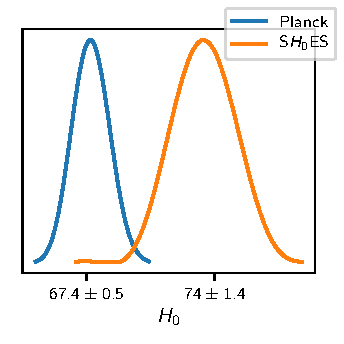
\includegraphics{./plots/H0.pdf}
            \end{overlayarea}
        \end{column}
    \end{columns}

    The multivariate $d$-dimensional equivalent to this tension would be:
    \[
        X^2_d = {(\mu_A - \mu_B)}^T{(\Sigma_A + \Sigma_B)}^{-1}(\mu_A-\mu_B),
    \]
    where $\Sigma$ is in general a covariance matrix.
\end{frame}

\begin{frame}
    \frametitle{Quantifying tension}
    \framesubtitle{non-Gaussians}
    \begin{figright}[0.4]{./figures/all_components.pdf}
        \begin{itemize}
            \item Things become less clear when distributions become ``banana like'' (\arxiv{1906.11628}),
        or worse, multimodal.
        \end{itemize}
    \end{figright}
    \begin{itemize}
        \item Many attempts to generalise the Gaussian case result in a parameterisation-dependent quantity.
    \end{itemize}
\end{frame}

\begin{frame}
    \frametitle{Quantifying tension}
    \framesubtitle{High-dimensional spaces}
    \centerline{%
    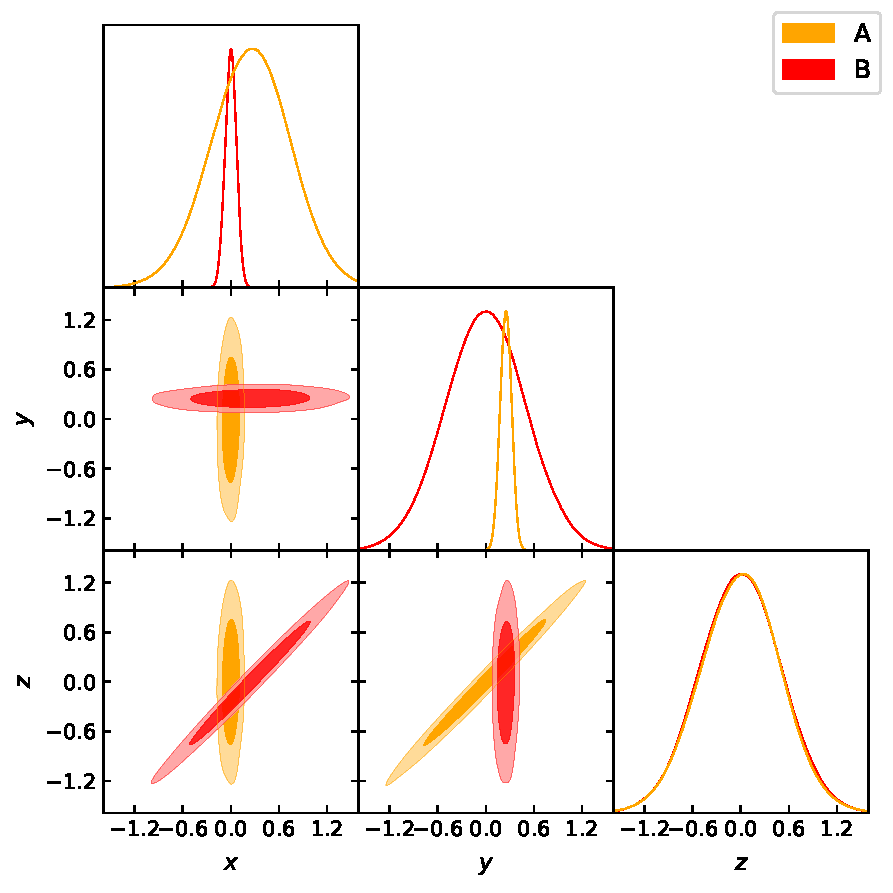
\includegraphics[width=0.49\textwidth]{./figures/tension.pdf}
    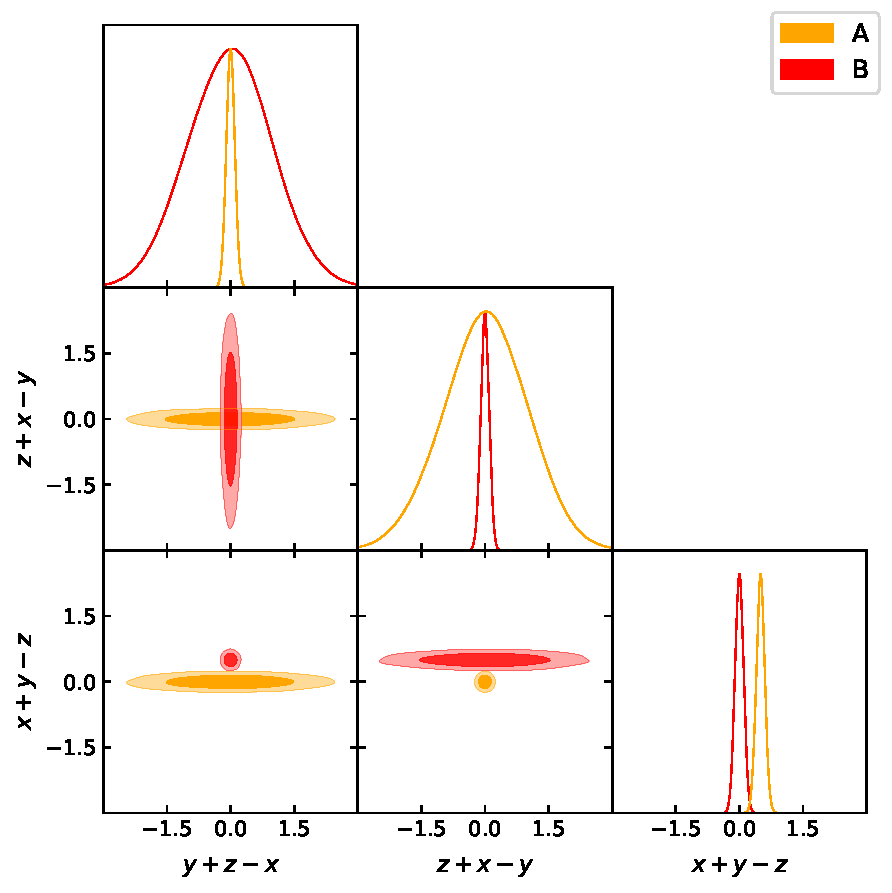
\includegraphics[width=0.49\textwidth]{./figures/tension_rotated.pdf}
    }
    \begin{itemize}
        \item In high dimensions, things can look good when projected into 2D.
        \item We need a systematic way of seeking out tension, without relying on inspired choices of parameters to reveal them
    \end{itemize}

\end{frame}

\begin{frame}
    \frametitle{The DES evidence ratio $R$}
    \begin{itemize}
        \item The Dark Energy Survey (\arxiv{1708.01530}) quantifies tension between two datasets $A$ and $B$ using the Bayes ratio:
            \[
                R = \frac{\mathcal{Z}_{AB}}{\mathcal{Z}_A \mathcal{Z}_B}
            \]
            where $\mathcal{Z}$ is the Bayesian evidence.
        \item Many attractive properties:
            \begin{itemize}
                \item Symmetry
                \item Parameterisation independence
                \item Dimensional consistency
                \item Use of well-defined Bayesian quantities
            \end{itemize}
        \item What does it mean?
    \end{itemize}
\end{frame}

\begin{frame}
    \frametitle{The meaning of the DES evidence ratio $R$}
    \begin{itemize}
        \item The Dark Energy Survey collaboration (\arxiv{1708.01530}) quantify tension between two datasets $A$ and $B$ using the Bayes ratio:
            \[
                R = \frac{\mathcal{Z}_{AB}}{\mathcal{Z}_A \mathcal{Z}_B} = \frac{P(A\cap B)}{P(A)P(B)} = \frac{P(A|B)}{P(A)} = \frac{P(B|A)}{P(B)}
            \]
        \item $R$ gives the relative change in our confidence in data $A$ in light of having seen $B$ (and vice-versa).
        \item $R>1$ implies we have more confidence in $A$ having received $B$.
        \item Like evidences, it is prior-dependent
        \item Increasing prior widths $\Rightarrow$ increasing confidence.
    \end{itemize}
\end{frame}

\begin{frame}
    \frametitle{The DES evidence ratio $R$: Prior dependency}
    {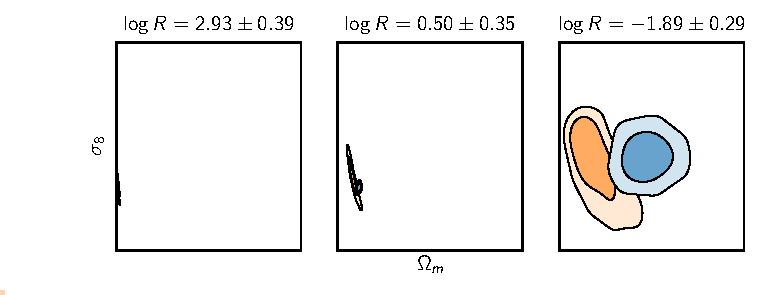
\includegraphics[trim=0.6in 0.3in 0in 0in]{./plots/prior_dependency.pdf}}
    \begin{itemize}
        \item What does it mean if increasing prior widths $\Rightarrow$ increasing confidence? 
        \item Wide priors mean {\em a-priori\/} the parameters could land anywhere.
        \item We should be proportionally more reassured when they land close to one another if the priors are wide
    \end{itemize}
\end{frame}

\begin{frame}
    \frametitle{How do we deal with the prior dependency in $R$?}
    \begin{description}
        \item[Option 1] Take the Bayesian route, accept the prior dependency, and spend time trying to justify why a given set of priors are ``physical''.
        \item[Option 2] Try to find a principled way of removing this prior dependency
    \end{description}
    \begin{itemize}
        \item One of the critical observations is that one can only hide tension by widening priors. Narrowing them will only ever show tension if it is present.
        \item If we could define ``Narrowest reasonable priors'' and find that $R<1$, then this would indicate tension.
    \end{itemize}
\end{frame}

\begin{frame}
    \frametitle{$R$: a Gaussian example}
    \begin{itemize}
        \item Given two Gaussians with parameter means $\mu_A,\mu_B$ and parameter covariances $\Sigma_A,\Sigma_B$ and a prior with volume $V_\pi$:
            \begin{align}
                \log R =& -\frac{1}{2} (\mu_A-\mu_B){(\Sigma_{A}+\Sigma_{B})}^{-1}(\mu_A-\mu_B)\nonumber\\
                & + \log V_\pi\nonumber -\log\sqrt{|2\pi(\Sigma_{A}+\Sigma_{B})|} 
            \end{align}
        \item Like evidence, $R$ composed of ``Goodness of fit'', and ``Occam factor''.
        \item Ideally want would remove this Occam factor (ratio of prior to posterior volume).
    \end{itemize}
\end{frame}

\begin{frame}
    \frametitle{KL divergence $\mathcal{D}$, Information $\mathcal{I}$, suspiciousness $S$}
    \begin{itemize}
        \item The KL divergence quantifies the compression from prior to posterior:
            \[
                \mathcal{D} = \int P(\theta|D) \log \frac{P(\theta|D)}{P(\theta)} d\theta = \left\langle\log\frac{\text{Posterior}}{\text{Prior}}\right\rangle_\text{Posterior}
            \]
        \item It bears many similarities to an Occam factor, for a Gaussian:
            \[
                \mathcal{D} =   \log V_\pi - \log \sqrt{|2\pi\Sigma|} - \frac{1}{2}d
            \]
        \item Can define equivalent of $R$ for KL divergence, the information ratio $\mathcal{I}$
            \begin{align}
                \log R &= \mathcal{Z}_{AB} -\mathcal{Z}_A - \mathcal{Z}_B \nonumber\\
                \log \mathcal{I} &= \mathcal{D}_A + \mathcal{D}_B - \mathcal{D}_{AB} \nonumber
            \end{align}
        \item Subtracting the two removes prior dependency, giving suspiciousness:
            \[
                \log S = \log R - \log \mathcal{I}
            \]
    \end{itemize}

\end{frame}

\begin{frame}
    \frametitle{Suspiciousness $S$}
    \begin{itemize}
        \item For a Gaussian:
            \[
                \log S = \frac{d}{2}  -\frac{1}{2} (\mu_A-\mu_B){(\Sigma_{A}+\Sigma_{B})}^{-1}(\mu_A-\mu_B).
            \]
        \item We thus find that our original idea for tension $X^2_d=d-2\log S$.
        \item However $S$ is composed of evidences $\mathcal{Z}$ and KL divergences $\mathcal{D}$, which are Gaussian-independent concepts.
        \item The only thing remaining to determine is $d$, the ``number of parameters''.
    \end{itemize}

\end{frame}

\begin{frame}
    \frametitle{Dimensionality $d$}
    \centerline{%
    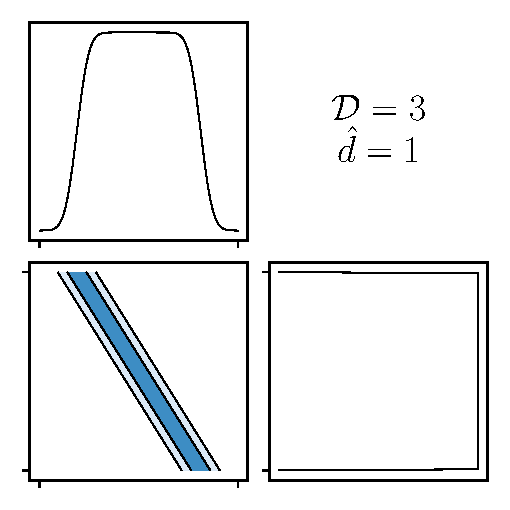
\includegraphics[width=0.49\textwidth]{./figures/dimensions_1.pdf}
    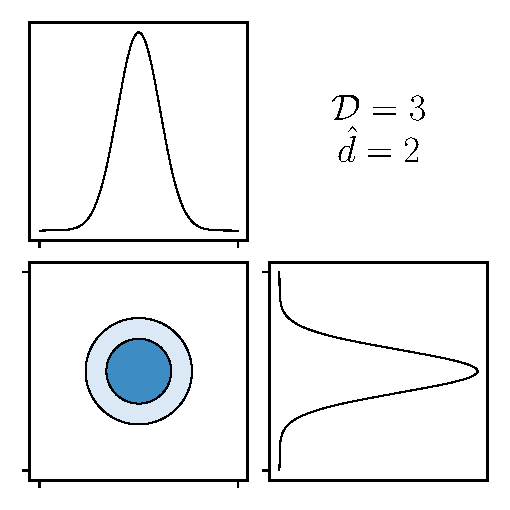
\includegraphics[width=0.49\textwidth]{./figures/dimensions_2.pdf}
    }
    \begin{itemize}
        \item Intuition should tell us that the $d$ we need is the effective number of parameters (i.e.\ should not include unconstrained ones).
        \item Like the evidence, or the KL divergence, this ``Model dimensionality'' should be a sought-after inference quantity.
    \end{itemize}

\end{frame}

\begin{frame}
    \frametitle{Dimensionality $\tilde{d}$}
    \begin{itemize}
        \item KL divergence is the mean of the Shannon information $I$:
            \begin{align}
                \mathcal{D} &= \int P(\theta|D) \log \frac{P(\theta|D)}{P(\theta)} d\theta = \left\langle\log\frac{\text{Posterior}}{\text{Prior}}\right\rangle_\text{Posterior}\nonumber\\
                I &= \log\frac{\text{Posterior}}{\text{Prior}}\nonumber
            \end{align}
        \item Model dimensionality proportional to variance of Shannon information:
            \[
                \frac{\tilde{d}}{2} = \text{var}\left(\frac{\text{Posterior}}{\text{Prior}}\right)_\text{Posterior}
            \]
        \item Examples from real data:
            \begin{align}
                \tilde{d}_\text{Planck} &= 15.8 \pm  0.3 &(21) \nonumber\\
                \tilde{d}_\text{DES} &= 14.0 \pm  0.3 &(26) \nonumber\\
                \tilde{d}_\text{BAO} &= 2.95 \pm  0.07 &(6) \nonumber\\
                \tilde{d}_\text{S$H_0$ES} &= 0.93 \pm  0.03 &(6) \nonumber
            \end{align}
    \end{itemize}

\end{frame}

\begin{frame}
    \frametitle{Headline results: $\Lambda$CDM}
    \begin{itemize}
        \item Can calibrate $X^2_d$ as on the same scale as $\chi^2_d$ to give a $p$-value-like quantity, termed ``Tension probability'' $p$, or $\sigma$
            \begin{align}
                \text{Planck 2015 vs BAO}:&      &p&=  42 \pm     4 \%        &\sigma& = 0.8\pm0.1\nonumber\\
                \text{Planck 2015 vs DES}:&      &p&=   3.2 \pm     1.0 \%    &\sigma& = 2.1\pm0.1\nonumber\\
                \text{Planck 2015 vs S$H_0$ES}:& &p&=   0.25 \pm     0.17 \%  &\sigma& = 3.1\pm0.3 \nonumber\\
                \text{Planck 2018 vs S$H_0$ES}:& &p&=   0.001 \pm     0.0001 \%  &\sigma& = 4.42\pm0.03\nonumber
            \end{align}
        \item Under this metric, S$H_0$ES is unambiguously inconsistent. BAO is consistent, and $DES$ is inconsistent, but only just. This is pleasingly similar to ones intuition.
		\item \arxiv{1902.04029}
    \end{itemize}
\end{frame}



\begin{frame}
    \frametitle{Headline results: $K\Lambda$CDM $\equiv\Lambda$CDM + $\Omega_K$}
    \begin{itemize}
        \item Cosmologies with curvature have different tension (\arxiv{1908.09139}):
            \begin{align}
                \text{Planck vs CMB lensing}:&      &p&=  1.3\pm 0.3 \% &\sigma& =2.5\pm0.1\nonumber\\
                \text{Planck vs BAO}:&      &p&=   0.25\pm 0.05 \% &\sigma& = 3.0 \pm 0.1 \nonumber
            \end{align}
		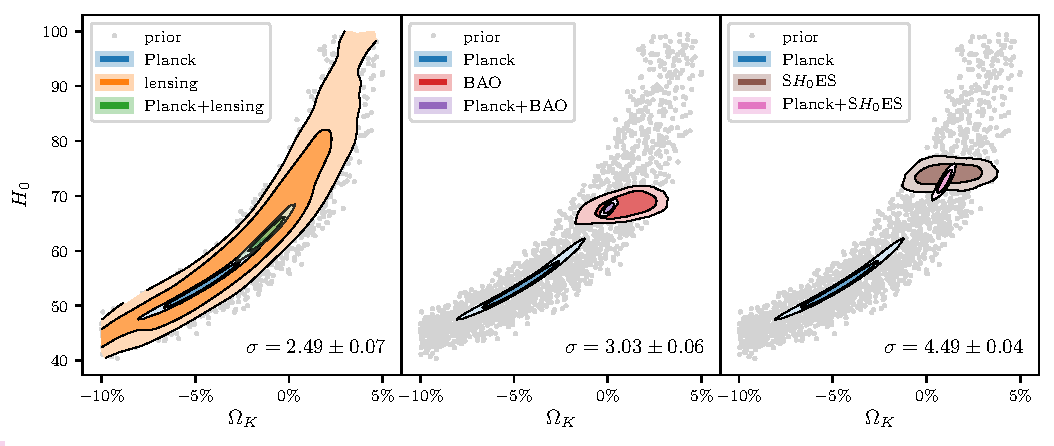
\includegraphics[width=\textwidth]{figures/omegak_H0.pdf}
        \item One should be suspicious about combining CMB lensing and Planck in curved models.
    \end{itemize}
\end{frame}

\begin{frame}
    \frametitle{Evidence: Is the universe curved?}
    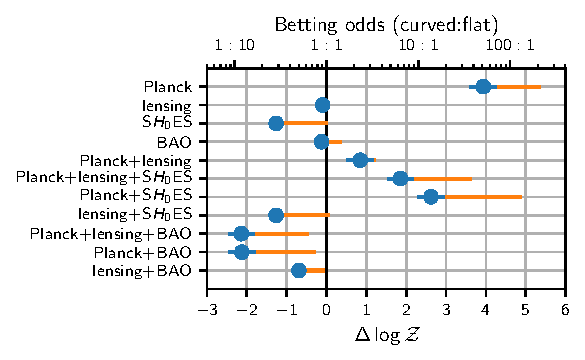
\includegraphics{figures/evidences.pdf}
    \begin{itemize}
        \item We only think the universe is flat because Planck+lensing and/or BAO tell us so, but these datasets are in tension.
        \item Planck alone tells us the universe is closed at 50:1
    \end{itemize}
\end{frame}

\begin{frame}
    \frametitle{What about $A_\mathrm{lens}$?}
    \begin{itemize}
        \item The Planck papers do discuss this, but phrase in terms of $A_\mathrm{lens}$
        \item $A_\mathrm{lens}$ is a ``fudge factor'' that artificially increases the effective smoothing by lensing on the primordial power spectrum if $A_\mathrm{lens}\ne 1$
        \item Planck CMB prefers $A_\mathrm{lens}\sim1.2$, lensing wants $A_\mathrm{lens}\sim1$ (can also be defined as a $\sim2\sigma$ tension)
        \item It is the same effect that causes the preference for closed universes.
    \end{itemize}
\end{frame}

\begin{frame}
    \frametitle{How do we fix curvature tension?}
    \begin{itemize}
        \item There could be several explanations:
        \item Systematic in Planck CMB
            \begin{itemize}
                \item Efstathiou \& Gratton's new likelihood looks like it may relax these tensions a little (results pending release of likelihood)
            \end{itemize}
        \item Systematic in Planck lensing
            \begin{itemize}
                \item The lensing likelihood includes a fiducial $\Lambda$CDM model.
                \item {\em In theory\/} this shouldn't matter, but re-doing the analysis with a different fiducial model is a mammoth task.
            \end{itemize}
        \item Statistical fluctuation?
            \begin{itemize}
                \item With tensions at $2$--$3\sigma$ there is always a possibility that we just got unlucky with our universe.
                \item There are a lot of these $2$--$3\sigma$ tensions in the Planck data. 
                \item If there were an explanation that resolved multiple tensions simultaneously then this could be decicive evidence for a new concordance model.
            \end{itemize}
        \item It may be that we need to wait for the next generation CMB experiment to resolve the issue (SO, LiteBird, PICO?, CORE?)
    \end{itemize}
\end{frame}

\begin{frame}
    \frametitle{Theory of curved universes}
    \begin{itemize}
        \item We generally work with flat cosmologies for a few reason
            \begin{enumerate}
                \item Data tell us it is (or does it?)
                \item Theory of inflation tells us it is (somewhat circular reasoning)
                \item The theory is \textbf{much} easier in flat cosmologies
            \end{enumerate}
        \item I've been interested in the effect of curvature at the start of inflation for a while
        \item Even small amounts of curvature can have observational effects on the primordial power spectrum
    \end{itemize}
\end{frame}


\begin{frame}
    \frametitle{History of curved universes}
    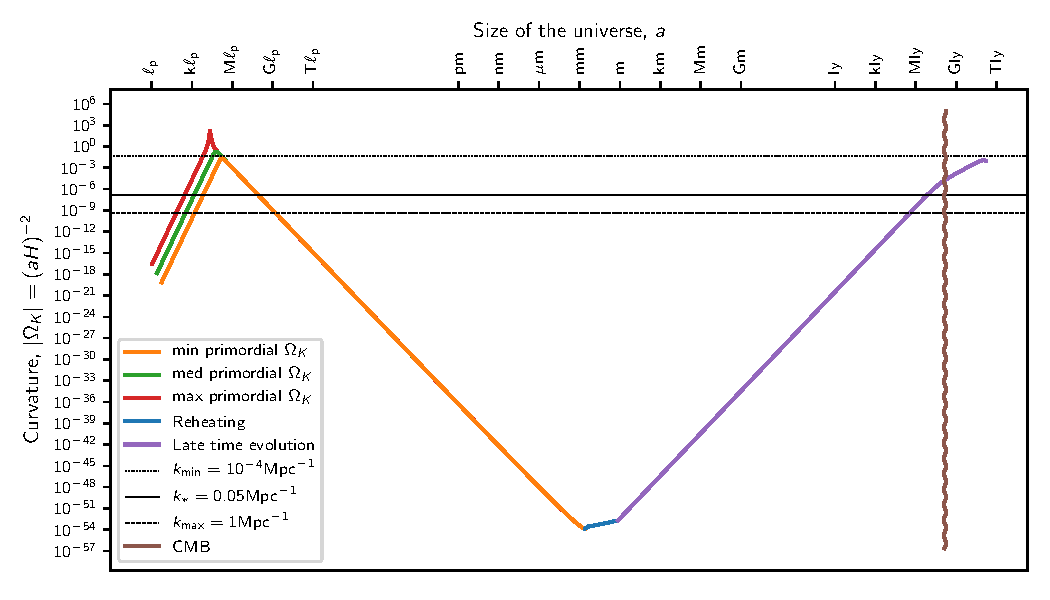
\includegraphics[width=\textwidth]{figures/history.pdf}
\end{frame}

\begin{frame}
    \frametitle{The primordial power spectrum}
    \begin{itemize}
        \item Inflationary theory interacts primarily with observation via the primordial power spectrum of curvature perturbations $\mathcal{P}_\mathcal{R}(k)$ (along with the tensor to scalar ratio $r$)
        \item $\Lambda$CDM assumes a near scale-invariant power spectrum 
            \[ \mathcal{P}_\mathcal{R}(k) = A_s {\left( \frac{k}{k_s} \right)}^{n_s-1} \]
        \item Inflation theories generally predict values of $(r,n_s)$ which can be compared with the phenomenological fit.
        \item $A_s$ is constrained by (amongst other things) the amplitude of the cosmic microwave background power spectrum
    \end{itemize}
\end{frame}
\begin{frame}
    \frametitle{Predictions from inflation}
    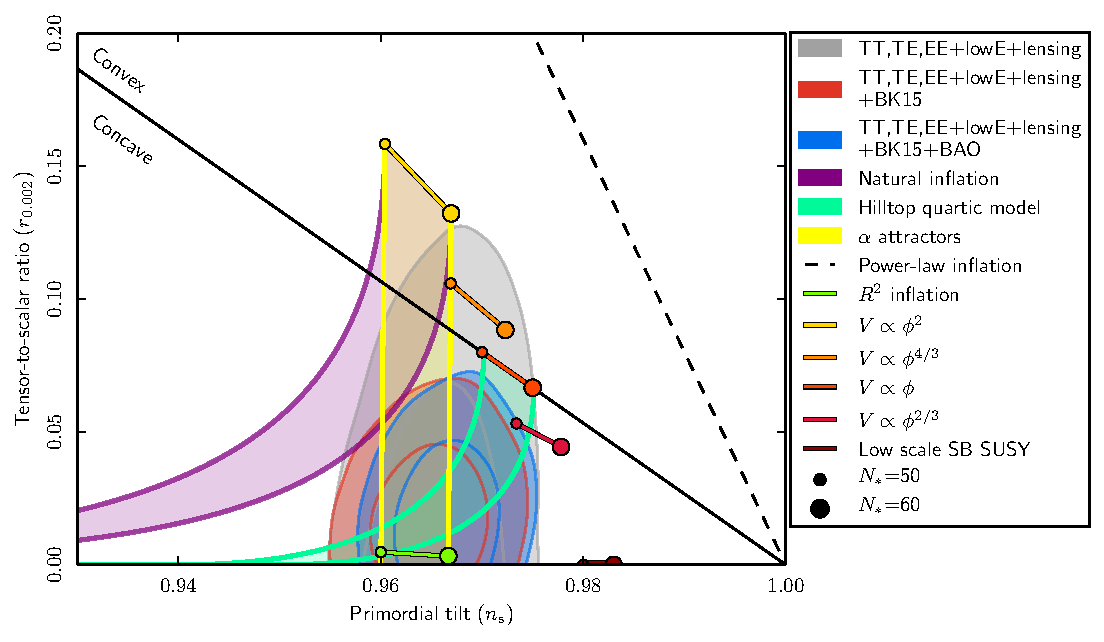
\includegraphics[width=\textwidth]{figures/inflation.pdf}
\end{frame}

\begin{frame}
    \frametitle{Primordial power spectrum computation}
    \begin{itemize}
        \item Background variables:
            \[ H^2 = \frac{1}{3}\left( \frac{1}{2}\dot\phi^2 + V(\phi) \right), \qquad 0=\ddot{\phi} + 3 H \dot{\phi} + \frac{d}{d\phi}V(\phi) \]
        \item Mukhanov variable $v= z\mathcal{R}$ ($z=a \dot{\phi}/H$) evolves according to:
            \[ 0 = v^{\prime\prime} + \left(k^2 - \frac{z^{\prime\prime}}{z}\right) v 
            \quad\Leftrightarrow\quad 0 = \mathcal{R}^{\prime\prime} + 2\frac{z^\prime}{z} \mathcal{R}^\prime + k^2 \mathcal{R} \]
    In terms of cosmic time $t$:
    \[ 
    0 = \ddot{\mathcal{R}} + \left(2\frac{z^\prime}{z}+H\right) \dot{\mathcal{R}} + k^2 \mathcal{R} 
\]
        \item During inflation $\eta\to\eta_*$ friction term $\to\infty$, mode freezes.
        \item Primordial power spectrum is $P_\mathcal{R}(k)\propto\lim_{\eta\to\eta_*} |\mathcal{R}|^2$
        \item Initial conditions for evolution set by quantum mechanics (more later)
    \end{itemize}
\end{frame}

\begin{frame}
    \frametitle{Mukhanov Sazaki equation in curved universes}

    \begin{itemize}
        \item In flat space:
        \begin{gather}
            H^2 = \frac{1}{3}\left( \frac{1}{2}\dot\phi^2 + V(\phi) \right), \qquad 0=\ddot{\phi} + 3 H \dot{\phi} + \frac{d}{d\phi}V(\phi), \qquad z=\frac{a \dot{\phi}}{H} \nonumber\\
            0 = \ddot{\mathcal{R}} + \left(2\frac{z^\prime}{z}+H\right) \dot{\mathcal{R}} + k^2 \mathcal{R} \nonumber
        \end{gather}
    \item With curvature ($K=-1,0,+1$):
        \begin{gather}
            H^2 = \frac{1}{3}\left( \frac{1}{2}\dot\phi^2 + V(\phi) \right) - \frac{K}{a^2}, \qquad 0=\ddot{\phi} + 3 H \dot{\phi} + \frac{d}{d\phi}V(\phi) \qquad z=\frac{a \dot{\phi}}{H}\nonumber\\
            \hspace{-10pt}0=\ddot{\mathcal{R}} + \frac{\left( H + \frac{2\dot z}{z} \right)\mathcal{D}^2 - \frac{3K H z^2}{2a^2}}{\mathcal{D}^2 - \frac{Kz^2}{2a^2}}\:\dot{\mathcal{R}}
            +\frac{K\left(1+\frac{z^2}{2a^2} - \frac{2}{H}\frac{\dot{z}}{z}\right)\mathcal{D}^2 + \frac{K^2z^2}{2a^2}-\mathcal{D}^4}{a^2(\mathcal{D}^2 - \frac{Kz^2}{2a^2})}\:\mathcal{R}\nonumber\\
            \mathcal{D}^2 = \nabla^2 +3K = -k^2 + 3K \nonumber
        \end{gather}
    \item  \arxiv{1907.08524}
    \end{itemize}
\end{frame}

\begin{frame}
    \frametitle{Primordial power spectrum}
    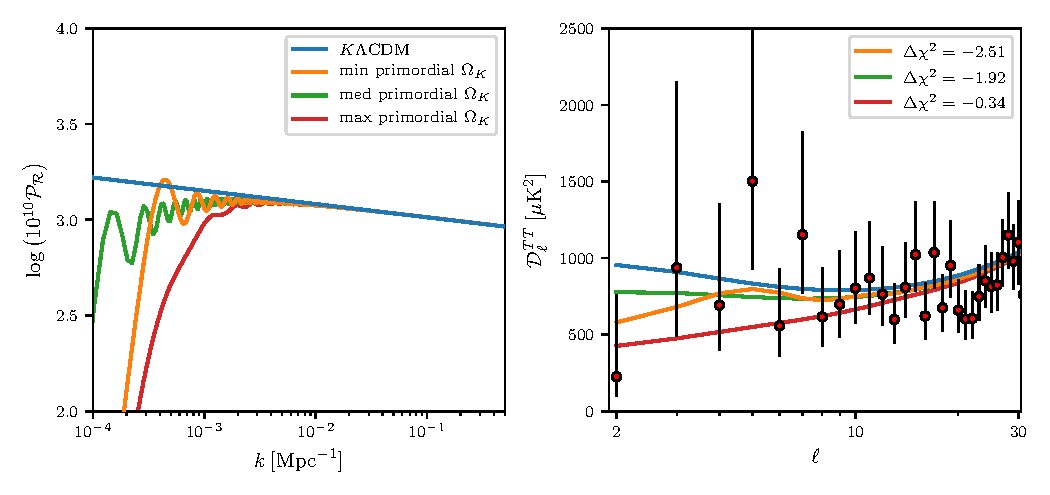
\includegraphics[width=\textwidth]{figures/BD.pdf}
\end{frame}

\begin{frame}
    \frametitle{Initial conditions in curved cosmologies}
    \begin{itemize}
        \item In the flat case, usuallyinitial conditions via ``Bunch Davies vacuum''  to initialise Mukhanov evolution:
            \[ v = \frac{1}{\sqrt{2k}} e^{-i k\eta}\]
        \item These are only valid for modes deep in the horizon $k\gg aH$, where the spacetime is de-Sitter (effectively Minkowski)
        \item In the curved case, the large spatial modes have $k\sim aH$
        \item Need new theory of quantum initial conditions for rapidly changing spacetimes.
        \item Instead of defining vacuum as ``particle-less'' (a relative concept), could define it in terms of ``lowest energy''
        \item Minimising the renormalised stress-energy yields observationally distinct initial conditions \arxiv{1607.04148}.
    \end{itemize}
\end{frame}


\begin{frame}
    \frametitle{Bunch Davies initial conditions}
    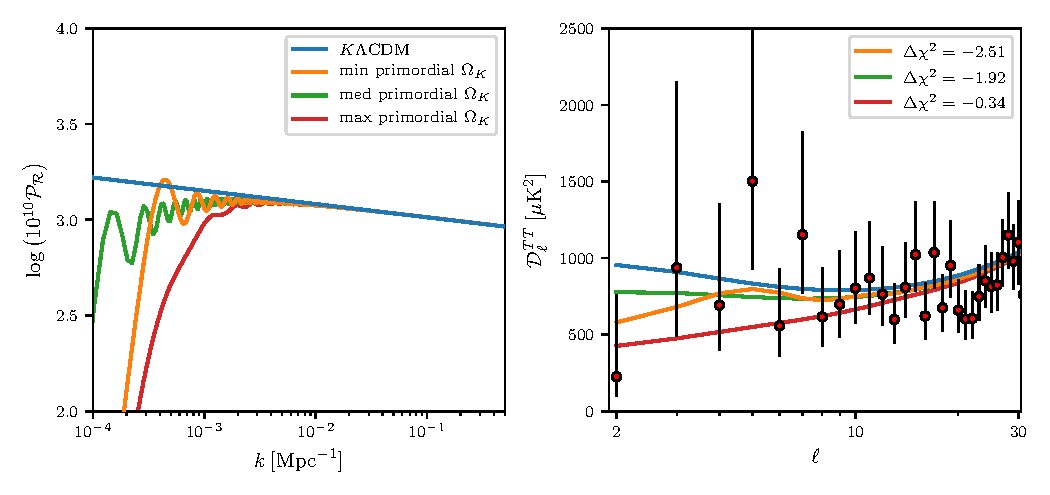
\includegraphics[width=\textwidth]{figures/BD.pdf}
\end{frame}


\begin{frame}
    \frametitle{Renormalised stress-energy initial conditions}
    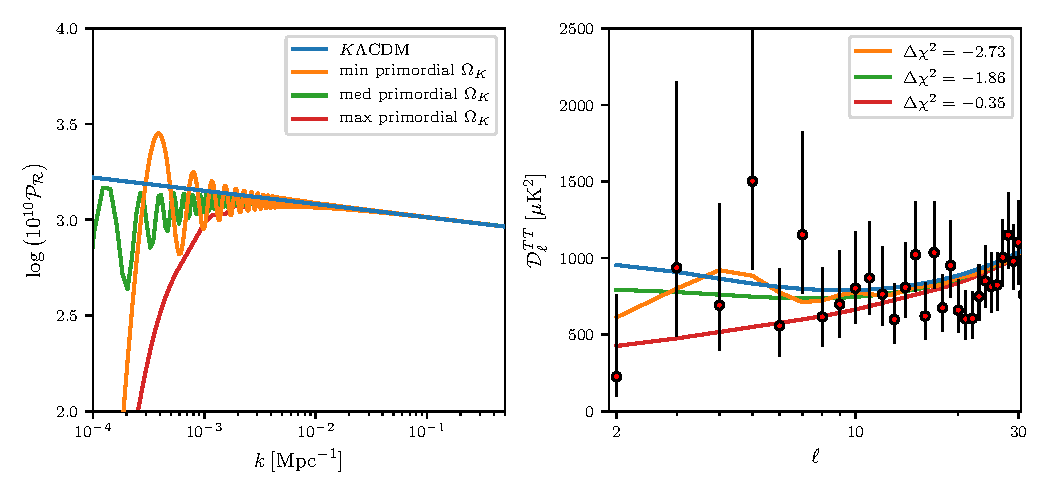
\includegraphics[width=\textwidth]{figures/RST.pdf}
\end{frame}


\begin{frame}
    \frametitle{Conclusions}
    \begin{itemize}
        \item The suspiciousness $S$ has become one of the standards for measuring tensions multiple simultaneous parameters.
        %\item The ``inference triple'' of $\mathcal{Z},\mathcal{D},\tilde{d}$ should be considered in all model comparison analyses (computed \texttt{anesthetic} package).
        \item Significant tensions remain for cosmologies that involve curvature, comparable in scale with other tensions that are discussed.
        \item Curvature+inflation yields a rich set of theoretical problems with potentially observable consequences.
    \end{itemize}
\end{frame}

\begin{frame}
    \frametitle{Extra slides}
\end{frame}



%\begin{frame}
%    \frametitle{Bayesian evidence $\mathcal{Z}$}
%    \begin{itemize}
%        \item Bayes theorem for parameter estimation:
%    \[
%    P(\theta|D) = \frac{P(D|\theta)P(\theta)}{P(D)} \quad\longrightarrow\quad \text{Posterior} = \frac{\text{Likelihood}\times\text{Prior}}{\text{Evidence}}
%    \]
%        \item Normalising constant $\equiv$ Bayesian evidence $\equiv$ $P(D)$ is hard to compute:
%    \[
%        P(D) = \int P(D|\theta)P(\theta) d\theta = \left\langle \text{Likelihood} \right\rangle_\text{Prior}
%    \]
%        \item Traditionally used to compare models using the same data
%        \item For DES, it is used to compare different data with the same model.
%        \item Computed using nested sampling (\texttt{MultiNest}, \texttt{PolyChord}, \texttt{dynesty}), simulated annealing (\texttt{emcee}), or from MCMC using \texttt{MCEvidence}.
%    \end{itemize}
%\end{frame}

\begin{frame}
    \frametitle{Bayesian evidence $\mathcal{Z}$: Prior dependency}
    \begin{itemize}
        \item Bayesian evidences are prior dependent:
            \[
                \mathcal{Z} = \int P(D|\theta)P(\theta) d\theta \approx \langle\text{Likelihood}\rangle_\text{Posterior} \times \frac{\text{Posterior volume}}{\text{Prior volume}}
            \]
        \item They balance ``goodness of fit'' via likelihood with ``complexity'' through Occam penalty.
        \item Models that include too many fine-tuned parameters are disfavoured, unless they provide a much better fit.
        \item Corollary: Unconstrained parameters are not penalised.
        \item Widen prior $\Rightarrow$ reduce evidence \\ (providing prior does not cut into posterior).
        \item Bayesians vs Frequentists $\leftrightarrow$ Feature vs Bug.
    \end{itemize}
\end{frame}

\begin{frame}
    \frametitle{The problem with Principle Component Analysis}

    \begin{figright}[0.6]{./plots/pca.pdf}
        \begin{itemize}
            \item Compute eigenvectors and eigenvalues of covariance matrix.
            \item These aim to describe ``directions'' in parameter space
            \item This procedure is not covariant:
        \end{itemize}
    \end{figright}
    \begin{quote}
        "Principal Component Analysis" is a dimensionally invalid method that gives people a delusion that they are doing something useful with their data. If you change the units that one of the variables is measured in, it will change all the "principal components"! It's for that reason that I made no mention of PCA in my book. I am not a slavish conformist, regurgitating whatever other people think should be taught. I think before I teach. David J C MacKay.

        \end{quote}
\end{frame}



\end{document}
